\chapter{Introduction}\label{ch:intro}

\section{Solar filament segmentation: what and why?}\label{sec:intro-what}
\epigraph{Nature uses only the longest threads to weave her patterns.}{Richard Feynman,
\emph{The Character of Physical Law} \citeyearpar{feynman1965}}

Photographed through a filter that passes only one red line of hydrogen, the Sun does not look
like a smooth bright ball. Its disk is covered with a mottled pattern of darker and brighter
cells, and across this pattern lie long, dark, thread-like structures called \keyterm{solar
filaments}. A filament is a cloud of cool, dense gas held up in the Sun's atmosphere by its
magnetic field~\citep{mackay2010,parenti2014}. Filaments can remain stable for days or weeks and
then erupt, and an eruption can be accompanied by a coronal mass ejection~\citep{webb2012}, a
cloud of magnetised plasma that may travel to the Earth.\footnote{A coronal mass ejection that reaches the Earth can disturb its magnetic field,
which in turn can affect satellites, radio communication and power grids.} Catalogues of filaments are therefore useful both to solar physicists and to
space-weather forecasters, and compiling them by hand is slow and tedious. This book is about a
machine-learning system that finds and outlines filaments automatically.

The precise task is set by a Kaggle competition, the Solar Filament Segmentation Challenge
2026~\citep{challenge}. The input is a single photograph of the Sun: a $2048\times2048$ grey
image taken through a filter that passes only the red \Ha{} line of hydrogen. The output is a
list of \keyterm{instance masks}, one binary image per filament, each marking the pixels that
belong to that filament, with the constraint that no pixel may belong to two masks. Each mask is
written as one row of a CSV file, in a compressed format called run-length encoding
(Section~\ref{sec:masks-rle}). A server compares these rows with masks drawn by human experts and
returns a single number between 0 and 1, the \keyterm{Panoptic Quality} (PQ), which we study in
Chapter~\ref{ch:metric}. Figure~\ref{fig:intro-task} summarises the setup. In the vocabulary of
computer vision, this is an \keyterm{instance segmentation} problem with a single object class;
we make the terminology precise in Section~\ref{sec:paradigms-kinds}.

\begin{figure}[t]
\centering
\begin{tikzpicture}[node distance=0.55cm]
  \node (in) {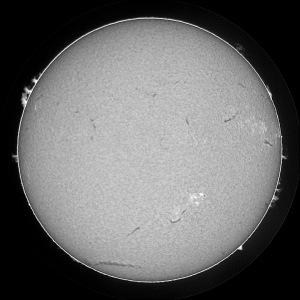
\includegraphics[width=2.1cm]{figures/thumb_input.png}};
  \node[note, below=0pt of in] {\Ha{} photograph\\ $2048\times2048$, grey};
  \node[box=vizblue, right=of in, minimum height=1.6cm, text width=2.3cm] (model)
       {\textbf{\color{inkprimary}segmentation model}\\[2pt] finds filaments and traces each one};
  \node[right=of model] (out) {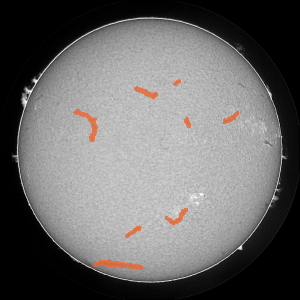
\includegraphics[width=2.1cm]{figures/thumb_output.png}};
  \node[note, below=0pt of out] {disjoint instance masks\\ (orange)};
  \node[box=vizorange, right=of out, minimum height=1.6cm, text width=2.0cm] (csv)
       {\textbf{\color{inkprimary}CSV}\\[2pt] one RLE row per filament};
  \draw[flow] (in) -- (model); \draw[flow] (model) -- (out); \draw[flow] (out) -- (csv);
  \node[box=vizaqua, below=1.25cm of csv, text width=2.0cm] (score) {\textbf{\color{inkprimary}PQ}\\ vs.\ each annotator};
  \draw[flow] (csv) -- (score);
\end{tikzpicture}
\caption{The task. A model turns one \Ha{} photograph into a set of non-overlapping masks, one per
filament. The masks are encoded as rows of a CSV file and scored with Panoptic Quality against
every annotator who labelled that photograph. \drawnin{book/chapters/ch01\_introduction.tex}}
\label{fig:intro-task}
\end{figure}

\subsection{Three questions in one}\label{sec:intro-questions}
It helps to recognise that the task combines three different questions.
\begin{enumerate}[leftmargin=*,itemsep=2pt]
\item \keyterm{Detection}: is there a filament at this location at all?
\item \keyterm{Delineation}: which pixels belong to it?
\item \keyterm{Identity}: is this dark region one filament, or two filaments that happen to
touch?
\end{enumerate}
A method can answer one of these questions well and another poorly. For example, the semantic
segmentation models of Chapter~\ref{ch:paradigms} delineate filaments reasonably well but have
no good way to decide identity; the YOLO models of Chapter~\ref{ch:yolo} detect filaments well
but draw masks that are slightly too wide; and the Mask2Former model of
Chapters~\ref{ch:transformers}--\ref{ch:submission} handles identity best of all but still misses
many faint filaments. The metric folds all three questions into one number, so a change in the
score seldom tells us, on its own, which of the three a change has improved. For this reason we
will often split the score into its parts (Section~\ref{sec:metric-sqrq}).

\section{Why the problem is hard}\label{sec:intro-hard}
Several properties of filaments make them difficult to segment. First, they are thin. The median
filament's bounding box is \LongPfifty{} pixels on its long side at the native resolution, but
its body is often only four or five pixels wide, so any step that reduces the resolution of the
image risks erasing it. Second, they are dark, but so is much else on the disk. The chromosphere
is covered by a network of dark and bright cells, and, pixel by pixel, a filament is no darker
than the network that surrounds it (we measure this in Section~\ref{sec:recall-physics}). Third,
they fade gradually into their surroundings, so where a filament ends is a matter of judgement,
and the image shows no sharp edge there. Fourth, a filament is often broken into several dark
patches that the eye groups into one object. Finally, near the edge of the disk (the
\keyterm{limb}), where the surface of the Sun curves away from us, filaments appear foreshortened
and dimmer.

The labels inherit all of these difficulties. Figure~\ref{fig:intro-annotators} shows one
photograph that three experts annotated independently. They agree about the large filaments, but
they draw \AnnotatorOne{}, \AnnotatorTwo{} and \AnnotatorThree{} filaments respectively, they
split and merge structures differently, and their outlines of the same filament differ by several
pixels. If we score one expert's masks against another expert's masks with the competition's
metric, we obtain a PQ of only about \HumanPQAll{} (Section~\ref{sec:metric-agreement}). This
fact shapes much of what follows: the target we are asked to predict is one person's judgement,
and different people judge differently. It does \emph{not} follow that \HumanPQAll{} is an upper
limit on what a model can score, and Section~\ref{sec:metric-agreement} explains why.

\begin{figure}[t]
\centering
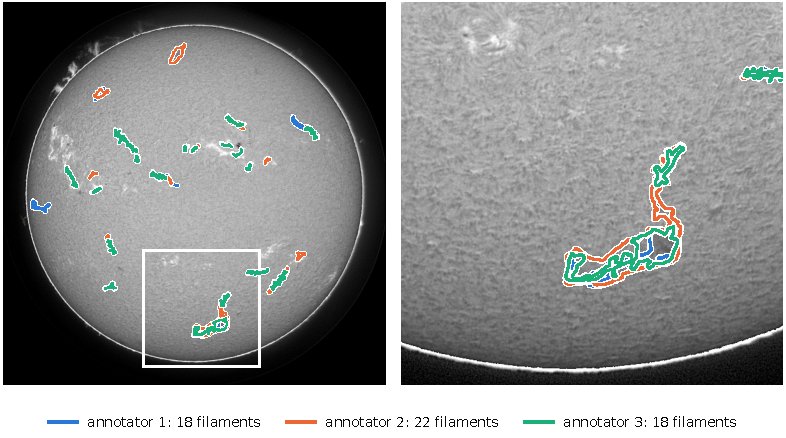
\includegraphics[width=\textwidth]{figures/fig_annotators.pdf}
\caption{One photograph labelled by three annotators working independently. Left: the full disk
with every annotator's outlines; the box marks the region shown on the right. Right: a
native-resolution zoom. The annotators agree that a filament is present, but not about its
extent or about how many pieces it consists of.
\generatedby{book/make\_book\_figures.py:fig\_annotators}}
\label{fig:intro-annotators}
\end{figure}

\section{The data}\label{sec:intro-data}
The competition supplies \AllPhotos{} training photographs with \AllRecords{} annotation
\keyterm{records}, where a record is one annotator's complete labelling of one photograph. Most
photographs were labelled once, but \TwiceAnnotated{} were labelled twice and \ThriceAnnotated{}
three times, which is why there are more records than photographs. In total the records contain
\AllFilaments{} annotated filaments. Each filament is stored as a polygon together with a traced
centre line called its \keyterm{spine}. The test set contains \TestPhotos{} photographs whose
labels are hidden. The public leaderboard scores roughly half of them, and the other half are
kept for the final ranking. Chapter~\ref{ch:data} describes the data in detail.

\section{The metric}\label{sec:intro-metric}
Panoptic Quality compares the predicted masks with the masks of one annotator at a time. A
predicted mask and an annotated mask \keyterm{match} if their intersection over union (IoU)
exceeds 0.5. Matched pairs are called \keyterm{true positives} (TP), unmatched predictions are
\keyterm{false positives} (FP), and unmatched annotations are \keyterm{false negatives} (FN).
The score is
\begin{equation}
\PQ = \frac{\sum_{(p,g)\in\TP}\IoU(p,g)}{|\TP| + \tfrac12|\FP| + \tfrac12|\FN|}
    = \underbrace{\frac{\sum_{\TP}\IoU}{|\TP|}}_{\SQ}\times
      \underbrace{\frac{|\TP|}{|\TP| + \tfrac12|\FP| + \tfrac12|\FN|}}_{\RQ},
\label{eq:intro-pq}
\end{equation}
where the counts are pooled over all annotation records. The first factor, the
\keyterm{segmentation quality} (SQ), is the mean IoU of the matched pairs; it measures how well
the filaments that were found have been outlined. The second factor, the \keyterm{recognition
quality} (RQ), is the $F_1$ score of the detections; it measures how many filaments were found and
how many spurious detections were made along the way. Chapter~\ref{ch:metric} analyses the
formula in detail, and we will see there that its structure explains many of our results.

\section{Previous work}\label{sec:intro-previous}
Automatic detection of filaments is older than deep learning. \citet{bernasconi2005} and
\citet{qu2005} described automated codes for full-disk \Ha{} images built from classical
image-processing operations, and \citet{schuh2014} evaluated and compared automated detection
methods. \citet{ahmadzadeh2019} trained a Mask R-CNN~\citep{maskrcnn} on images from the Big Bear
Solar Observatory, using as labels the output of an existing automatic detector stored in the
Heliophysics Events Knowledgebase, and noted that any error in those labels is inherited by a
model that learns from them. \citet{zhu2019} trained a U-Net~\citep{unet} and tested it on 60 manually
corrected images from the same observatory, and \citet{guo2022} used deep networks
to detect filaments and to classify them. \citet{diercke2024} trained a YOLO detector on labelled
images from one telescope, used it to find filaments in the whole GONG archive, and then used the
resulting boxes to train a U-Net that labels filament pixels; the method is meant to work on
images from several observatories.

The MAGFiLO dataset~\citep{magfilo}, from which the competition's data are drawn, gave the field a
common set of expert annotations of GONG images. \citet{edgeattnet} trained a U-Net with an
edge-guided attention layer on it, aiming to capture the thin side branches, or barbs, from which
a filament's chirality is determined, and \citet{hao2026sabr} studied losses that reward the
coverage of thin annotated structures. Other recent work uses other data: \citet{hu2026morden}
built their own datasets for a multiscale semantic segmentation model, \citet{reche2026} built a
new dataset of GONG images for a transformer detector followed by a U-Net, and
\citet{srivastava2026} combined observations from several instruments using weak labels.
\citet{hu2026review} review the development of these methods, from manual catalogues to deep
learning.

As far as we know, none of these papers reports Panoptic Quality, and none of their numbers can be
compared directly with the numbers in this book. The papers that we could check report pixel-level
measures (accuracy, the Dice coefficient or IoU), measures of how well thin structures are covered,
or detection scores under their own matching rules, and each evaluates on its own images. Pixel
accuracy is the least informative of these: filament pixels make up only about one per cent of the
disk (Section~\ref{sec:par-loss}), so a model that marks nothing is already about 99\% accurate.
The closest comparison we know of is with \citet{edgeattnet}. Their pairwise IoU, computed over
overlapping pairs of predicted and annotated filaments, is 0.645 on their own test split of 99
MAGFiLO images, and the organisers' notebook reports a mean IoU of \MeanIoUOverlap{} over
overlapping pairs for our final model on our validation split (Section~\ref{sec:sub-eval}). Even
these two numbers are not comparable. They come from different images, and a mean taken only over
overlapping pairs ignores both the filaments that a model misses and the ones that it invents,
which Panoptic Quality counts (Chapter~\ref{ch:metric}).

\section{A short history of our attempts}\label{sec:intro-journey}
Figure~\ref{fig:intro-progress} plots the public score of every submission in the order in which
they were made, and Table~\ref{tab:intro-milestones} lists the changes that moved it. The score
rose in a few large steps separated by long periods without progress. Each large step came from a
change in \emph{what} we modelled or \emph{how} we measured it, such as predicting at the native
resolution or correcting a systematic bias in the training masks. Tuning a hyperparameter never
produced a large step: the one step in the table that came from tuning, the lower confidence
threshold of exp062, was worth a single hundredth. Most of the experiments described in this book
belong to the periods without progress.

\begin{figure}[t]
\centering
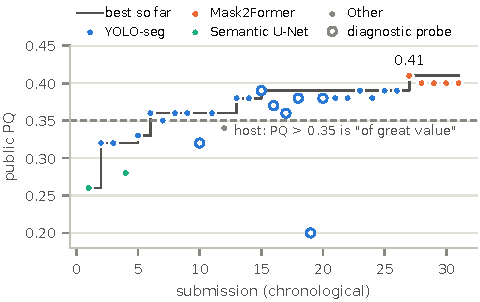
\includegraphics[width=0.8\textwidth]{figures/fig_progress.pdf}
\caption{Public PQ of all \Submissions{} submissions in the order in which they were made,
coloured by model family. Hollow markers are diagnostic probes, which we submitted to learn
something about the leaderboard; we did not expect them to raise the score.
\generatedby{paper/make\_figures.py:figure\_progress}}
\label{fig:intro-progress}
\end{figure}

\begin{table}[t]
\centering\small
\caption{The changes that moved the public score. Validation PQ is measured on our fixed
validation split (Chapter~\ref{ch:validation}).}
\label{tab:intro-milestones}
\begin{tabularx}{\textwidth}{@{}lXcc@{}}
\toprule
experiment & change & validation & public \\
\midrule
exp001 & U-Net++ semantic segmentation, then connected components & 0.2957 & 0.26 \\
exp002 & YOLO11m-seg instance segmentation trained at 1280 px & 0.3736 & 0.32 \\
exp002 & same weights, inference at the native 2048 px & 0.4064 & 0.33 \\
exp005 & erode every predicted mask by one pixel & 0.4404 & 0.36 \\
exp037 & eight-view test-time augmentation with fusion & 0.4571 & 0.38 \\
exp062 & lower emission confidence (0.35) with fusion & 0.4559 & 0.39 \\
exp119 & two-architecture YOLO ensemble & 0.4681 & 0.39 \\
\textbf{exp139} & \textbf{Mask2Former at native resolution, one view} & \textbf{0.4705} & \textbf{0.41} \\
\bottomrule
\end{tabularx}
\end{table}

Figure~\ref{fig:intro-map} groups the approaches we tried into four families and shows where
each is described. It can be read as a table of contents organised by idea.

\begin{figure}[t]
\centering
\begin{tikzpicture}[
  fam/.style={box=#1, text width=2.35cm, minimum height=0.9cm,
              execute at begin node={\hyphenpenalty=10000}},
  leaf/.style={font=\sffamily\scriptsize, text=inksecondary, align=left, text width=2.4cm,
               anchor=north},
  node distance=0.18cm]
  \node[fam=vizaqua] (dense) at (0,0) {\textbf{\color{inkprimary}Dense\\ segmentation}\\ Ch.~\ref{ch:paradigms}};
  \node[fam=vizblue] (yolo) at (2.9,0) {\textbf{\color{inkprimary}YOLO\\ instances}\\ Ch.~\ref{ch:yolo}--\ref{ch:tta}};
  \node[fam=vizyellow] (post) at (5.8,0) {\textbf{\color{inkprimary}Fixing\\ masks}\\ Ch.~\ref{ch:post}};
  \node[fam=inkmuted] (recall) at (8.7,0) {\textbf{\color{inkprimary}Finding\\ misses}\\ Ch.~\ref{ch:recall}};
  \node[leaf] at (0,-0.85) {U-Net++ @512: 0.26\\ U-Net @1024: 0.28\\ spine seeding: $\pm$0\\ centre/offset: $\le$0};
  \node[leaf] at (2.9,-0.85) {train 1280: 0.32\\ infer 2048: 0.33\\ 1 px erosion: 0.36\\ D4 fusion: 0.38--0.39\\ YOLOv8l @2048: 0.39\\ 2-model ensemble: 0.39};
  \node[leaf] at (5.8,-0.85) {refiners: $-$0.008, $-$0.031\\ logit cut, SAM2: $\le$0\\ edge snapping: harmful\\ split, grow: 13--34\%\\ of oracle ceilings};
  \node[leaf] at (8.7,-0.85) {verifiers: $\le$+0.002\\ crop CNN: chance\\ physics proposals keep\\ 26\% of the disk\\ semantic pruning: 0.39};
  \node[fam=vizorange, text width=10.9cm] (m2f) at (4.35,-4.25)
       {\textbf{\color{inkprimary}Mask2Former at native resolution} (Ch.~\ref{ch:transformers}--\ref{ch:submission}):
        first attempt at 1024 px 0.30 validation; proper training 0.4705 validation, \textbf{0.41 public}};
\end{tikzpicture}
\caption{The approaches we tried, grouped by family, with the chapter that describes each. Numbers
are public PQ unless they are marked as a change in validation PQ.
\drawnin{book/chapters/ch01\_introduction.tex}}
\label{fig:intro-map}
\end{figure}

\section{The final model}\label{sec:intro-winner}
Our final model is a single \keyterm{Mask2Former} network~\citep{mask2former} with a Swin-S
backbone~\citep{swin}, trained for 50 epochs on one H100 GPU, and its submission scores
\BestPublic{} on the public leaderboard. Three
design decisions account for most of its performance, and later chapters support each of them
with measurements.
\begin{enumerate}[leftmargin=*,itemsep=2pt]
\item \textbf{Native resolution.} We never shrink the photograph. Mask2Former predicts masks at a
quarter of the resolution of its input, so when the input is the native $2048\times2048$ image
the masks lie on a grid of cells four pixels wide. Section~\ref{sec:train-resolution} shows that a
grid this fine can represent the annotated masks almost perfectly, whereas the coarser grid that
results from a shrunken input cannot.
\item \textbf{Set prediction.} Mask2Former proposes a fixed set of 100 candidate objects, and it is
trained, through a one-to-one matching between candidates and annotated filaments, to propose each
filament only once. As a result it rarely splits a filament into several masks or merges several
filaments into one (Section~\ref{sec:tr-detr}).
\item \textbf{A validation procedure that agrees with the leaderboard.} Our evaluation code
reproduces the organisers' scoring code to nine decimal places, so a decision taken on our
validation split is a decision about the quantity that the leaderboard measures
(Section~\ref{sec:sub-eval}).
\end{enumerate}
On our validation split the model scores a PQ of \HostPQ{}, with a 95\% bootstrap interval of
\PQLow{}--\PQHigh{} over resamples of the validation photographs. Chapter~\ref{ch:submission}
examines what it does well and what it still misses.

\section{How to read this book}\label{sec:intro-read}
Readers who only want to understand the final model can read Chapters~\ref{ch:metric},
\ref{ch:transformers}, \ref{ch:training} and~\ref{ch:submission} after this one. Readers who want
to understand how we arrived at that model should read the chapters in order, since each of
Chapters~\ref{ch:paradigms} to~\ref{ch:recall} ends with the measurements that closed one line of
work and motivated the next. Readers who want to use the masks for solar physics should read
Chapters~\ref{ch:data}, \ref{ch:metric} and~\ref{ch:submission}, which describe the data, what the
score measures, and which filaments the final model finds and which it misses.
Chapter~\ref{ch:lessons}, on experimental method, is best read last.

\section*{Exercises}
\begin{exercise}{Reading the headline numbers}
The deployed model has \NumTP{} true positives, \NumFP{} false positives and \NumFN{} false
negatives on the validation split, and its SQ is \ValSQ{}. Use Equation~\eqref{eq:intro-pq} to
compute its RQ and PQ, and compare your answers with Table~\ref{tab:intro-milestones}.
\end{exercise}

\begin{exercise}{Records and photographs}
Load \file{data/MAGFiLO\_1.0\_Annotations\_kaggle2026\_train.json} with Python's \texttt{json}
module. Count the entries in its \texttt{images} list and the number of distinct values of their
\texttt{file\_name} field. Explain why the two counts differ, and find a photograph that was
labelled three times.
\end{exercise}

\begin{exercise}{Regenerating a figure}
Run \file{book/make\_book\_figures.py} with the arguments given in its docstring. Then modify
\texttt{fig\_annotators} so that it selects the three-annotator photograph with the \emph{fewest}
filaments, and describe how the annotators' disagreement changes.
\end{exercise}

\begin{exercise}{Finding the evidence}
Choose one row of Table~\ref{tab:intro-milestones}. Find the corresponding experiment in
\file{docs/leaderboard-analysis.md} or \file{docs/ACTIVE\_EXPERIMENT.md}, and write down the TP,
FP and FN counts behind its validation score.
\end{exercise}
